\subsection{\texorpdfstring{\(C^{\Lambda}\) 的紧子集上的连续函数}{C\^{}\{Lambda\} 的紧子集上的连续函数}}

设 \(\Lambda\) 为一个集合，X 为 \(\mathbf{C}^{\Lambda}\) 的一个紧子集。我们用 P(X) 表示 \(\mathcal{C}(\mathrm{X})\) 的幺 Banach 子代数，它由 X 上这样的函数组成：它们是 \(\mathbf{C}^{\Lambda}\) 上多项式函数在 X 上的一致极限。坐标函数 \(z_{\lambda}|\mathrm{X}\) 拓扑地生成 P(X)，且 P(X) 分离 X 的点。设 Y 为 X 的多项式凸包（I，第 45 页，定义 4）。由于

\[
\sup _ {z \in \mathrm{Y}} | p (z) | = \sup _ {z \in \mathrm{X}} | p (z) |
\]

（参见 I，第 44 页，第 7 节）对所有 \(p \in \mathbf{C}[(\mathrm{X}_{\lambda})_{\lambda \in \Lambda}]\) 成立，X 上一致收敛的多项式序列便可唯一扩张为 Y 上一致收敛的多项式序列。因此存在唯一的从 P(X) 到 P(Y) 上的等距同构，它对每个坐标函数 \(z_{\lambda}\) （\(\mathbf{C}^{\Lambda}\) 上的坐标函数），把 \(z_{\lambda}|X\) 映为 \(z_{\lambda}|Y\) 。我们称这个同构为典范同构。

命题 4.　设 X 为紧空间。设 B 为 \(\mathcal{C}(\mathrm{X})\) 的幺 Banach 子代数，赋以诱导范数，且分离 X 的点。我们把 X 等同于 \(\mathrm{X(B)}\) 的一个闭子集（I，第 142 页，命题 1，d)）。设 \((x_{\lambda})_{\lambda \in \Lambda}\) 为 B 中拓扑地生成幺代数 B 的元素所成的族。我们考虑交换图

\pandocbounded{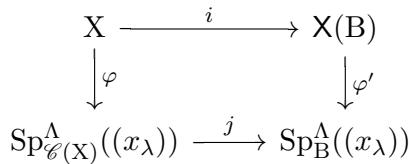
\includegraphics[keepaspectratio]{images/part001_f1662ccb.jpg}}

其中 \(\varphi\) 与 \(\varphi'\) 是由族 \((x_{\lambda})_{\lambda \in \Lambda}\) 所定义的映射（参见 I，第 41 页，第 6 节），而 \(i\) 与 \(j\) 是典范单射。则：

\begin{enumerate}
\def\labelenumi{\alph{enumi})}
\item
  映射 \(\varphi\) 与 \(\varphi'\) 是同胚；
\item
  联合谱 \(\mathrm{Sp}_{\mathrm{B}}^{\Lambda}((x_{\lambda}))\) 是 \(\mathrm{Sp}_{\mathcal{C}(\mathrm{X})}^{\Lambda}((x_{\lambda}))\) 的多项式凸包；
\item
  映射 \(\varphi\) 把 \(\mathcal{C}(\mathrm{X})\) 映为 \(\mathcal{C}(\mathrm{Sp}_{\mathcal{C}(\mathrm{X})}^{\Lambda}((x_{\lambda})))\) ，把 B 映为 \(\mathrm{P}(\mathrm{Sp}_{\mathcal{C}(\mathrm{X})}^{\Lambda}((x_{\lambda})))\) ；
\item
  映射 \(\varphi^{\prime}\) 把 \(\mathcal{G}_{\mathrm{B}}(\mathrm{B})\) 映为 \(\mathrm{P}(\mathrm{Sp}_{\mathrm{B}}^{\Lambda}((x_{\lambda})))\) ；
\item
  映射 \(\varphi\) 与 \(\varphi'\) 把 \(\mathcal{G}_{\mathrm{B}}\) 映为从 \(\mathrm{P}(\mathrm{Sp}_{\mathcal{C}(\mathrm{X})}^{\Lambda}((x_{\lambda})))\) 到 \(\mathrm{P}(\mathrm{Sp}_{\mathrm{B}}^{\Lambda}((x_{\lambda})))\) 上的典范同构。
\end{enumerate}

映射 \(\varphi\) 与 \(\varphi'\) 是连续且满射的（I，第 41 页，第 6 节）。映射 \(\varphi'\) 由 I，第 43 页，命题 12 的断言 \(a\) ）是同胚，且 \(i\) 是单射，因此 \(\varphi\) 是单射。于是 \(\varphi\) 与 \(\varphi'\) 都是同胚。

设 \(X_{1} = \mathrm{Sp}_{\mathcal{C}(X)}^{\Lambda}((x_{\lambda}))\) 。由 I，第 46 页，命题 14，\(X_{1}\) 的多项式凸包是 \(Y_{1} = \mathrm{Sp}_{\mathrm{B}}^{\Lambda}((x_{\lambda}))\) 。

对每个 \(\lambda\in\Lambda\) ，设 \(z_{\lambda}\) 是 \(\mathbf{C}^{\Lambda}\) 上相应的坐标函数。映射 \(\varphi\) 把 \(x_{\lambda}\) 映为 \(z_{\lambda}|X_{1}\) ，\(\varphi'\) 把 \(\mathcal{G}_{\mathrm{B}}(x_{\lambda})\) 映为 \(z_{\lambda}|Y_{1}\) 。因此 \(\varphi\) 把 B 映到 \(\mathrm{P}(X_{1})\) 上，\(\varphi'\) 把 \(\mathcal{G}_{\mathrm{B}}(B)\) 映到 \(\mathrm{P}(Y_{1})\) 上。最后，\(\varphi\) 与 \(\varphi'\) 把 \(\mathcal{G}_{\mathrm{B}}\) 映为从 \(\mathrm{P}(X_{1})\) 到 \(\mathrm{P}(Y_{1})\) 上的典范同构。

推论 1.　设 \(\Lambda\) 为一个集合，X 为 \(\mathbf{C}^{\Lambda}\) 的紧子集。我们把 X 等同于 \(\mathsf{X}(\mathrm{P}(\mathrm{X}))\) 的一个子集（I，第 142 页，命题 1，d)）。设 \((z_{\lambda})_{\lambda \in \Lambda}\) 为 \(\mathbf{C}^{\Lambda}\) 上坐标函数所成的族。

\begin{enumerate}
\def\labelenumi{\alph{enumi})}
\item
  映射 \(\theta\) 从 \(\mathrm{X}(\mathrm{P}(\mathrm{X}))\) 到 \(\mathrm{Sp}_{\mathrm{P}(\mathrm{X})}^{\Lambda}((z_{\lambda}))\) 上、由族 \((z_{\lambda})\) 所定义，它是从 \(\mathrm{X}(\mathrm{P}(\mathrm{X}))\) 到多项式凸包 \(Y\) （\(X\) 的多项式凸包）上的同胚。它在 \(X\) 上的限制是 \(X\) 的恒等映射；
\item
  对每个函数 \(f \in \mathrm{P}(\mathrm{X})\) ，同胚 \(\theta\) 把扩张 \(\mathcal{G}_{\mathrm{P}(\mathrm{X})}(f)\) （\(f\) 到 \(\mathrm{X}(\mathrm{P}(\mathrm{X}))\) 上的扩张）变换为扩张 \(\widetilde{f}\) （\(f\) 到 \(\mathrm{Y}\) 上的扩张）。映射 \(f \mapsto \widetilde{f}\) 是从 \(\mathrm{P}(\mathrm{X})\) 到 \(\mathrm{P}(\mathrm{Y})\) 上的典范同构。
\end{enumerate}

在命题 4 中取 B = P(X) 及 \(x_{\lambda} = z_{\lambda}\) 。则 \(\varphi\) 变成恒等映射，\(\varphi'\) 变成映射 \(\theta\) 。于是推论的断言就归结为同前处的断言。

推论 2.　设 \(\Lambda\) 为一个集合，\(X \subset \mathbf{C}^{\Lambda}\) 为紧集。若 \(X\) 连通，则它的多项式凸包连通。

若 X 连通，则 \(\mathcal{C}(\mathrm{X})\) 从而 \(\mathrm{P}(\mathrm{X})\) 的幂等元只有 0 和 1（I，第 79 页，命题的推论）。因此，空间 \(\mathrm{X}(\mathrm{P}(\mathrm{X}))\) 是连通的（同前）；而这个集合同胚于 X 的多项式凸包（推论 1，a)）。

